\pdfoutput=1
\documentclass[11pt]{article}
\usepackage[margin=1in]{geometry}
\usepackage{times}
\usepackage{booktabs}
\usepackage{graphicx}
\usepackage{amsmath}
\usepackage{url}
\usepackage{hyperref}
\usepackage{xcolor}
\usepackage{caption}
\usepackage{microtype}
\setlength{\emergencystretch}{2em}
\hypersetup{colorlinks=true, linkcolor=black, citecolor=blue!60!black, urlcolor=blue!60!black,
  pdftitle={Typed, Calibrated Decisions for an Offline Network-Management Agent}, pdfauthor={Krish Viswanathan}}
\newcommand{\todo}[1]{\textcolor{red}{[#1]}}

\title{Typed, Calibrated Decisions for an Offline Network-Management Agent:\\
\large Serving the System One Idea Next to a 4B Model on an Embedded NPU}
\author{Krish Viswanathan}
\date{September 2026 --- preprint, v0.1}

\begin{document}
\maketitle

\begin{abstract}
An offline network-management assistant runs a 4-billion-parameter instruction-tuned model on
an embedded NPU (Qwen3-4B-Instruct-2507, W4A16, Qualcomm QCS9075) and turns an operator's
sentence into one tool call against a managed PoE switch; a human confirms every write. The
generative path is accurate on canonical phrasing (92--97\% end-to-end) and weaker on
paraphrases (77.4\%; 61.5\% on indirect phrasing), but two properties matter more than the
headline: its misses are structured, several of them dangerous (cut PoE power versus shut the
interface; one access VLAN versus a trunk), and it emits no probability, so the confirm gate
cannot tell a confident call from a coin flip. On the compiled NPU serving path there are no
logits to read. We borrow the interface of TypeSafe's Jev --- typed questions (yes/no, one of
$K$, ordered levels) over a state, answered in one pass with calibrated probabilities --- and
serve it locally on the CPU next to the generative agent. We compare four realizations on one
labeled workload of 519 operator requests (65 seeds, 195 style-controlled paraphrases, 259 rows
authored for the study): a next-token readout of the resident 4B over single-token labels via
\texttt{llama-server}, three open encoder decision models zero-shot (151M--421M), a 150M encoder
fine-tuned on the domain, and rules. We measure accuracy per phrasing style, calibration before
and after out-of-fold temperature scaling (folds grouped by seed request), order sensitivity under
option rotation, selective accuracy at the thresholds Jev recommends, and how many of the
generative model's \emph{real} misses a ``does this proposal match the request'' question flags.
The readout is not a better router (84.6\% on a 24-way command question vs the generative call's
83.1\%), and its raw confidence is unusable (23 of 40 errors above $p=0.9$; 29--36\% of answers
flip under option reordering on adversarial rows), but once temperature-scaled and
rotation-averaged it gives the gate an AUROC-0.95 check that flags 15 of the agent's 20 real
dangerous confusions at $p<0.5$ while false-flagging 30 of 151 correct proposals, and admits 1 of
156 dangerous synthetic swaps; on the board's CPU it costs 1.3\,s per router question and 3\,s per
gate question with the question prefix cached. The zero-shot open reproductions are at chance on
the gate and collapse above about six options. A 150M encoder fine-tuned on $\sim$2,000 rows
with the question order shuffled becomes the better router than the readout on identical
held-out rows (tool 88.1\% vs 84.9\%, command 77.8\% vs 69.8\%) at 126\,ms per question on the
board's CPU, but no encoder variant learns the gate (AUROC 0.53--0.65): the division of labour
is an encoder for the per-turn router and a decoder readout for the per-write gate. We release
the code, the dataset and the result receipts.
\end{abstract}

\section{Introduction}

Small language models now drive tool-calling agents on embedded accelerators. On a Qualcomm
QCS9075 board, a 4B instruction-tuned model compiled to the Hexagon NPU answers an operator in
6--7\,s per turn and reaches 92--97\% end-to-end accuracy on a 65-case tool-calling benchmark
against a live managed switch~\cite{lancefindings}. That accuracy is measured on canonical
phrasing. On a 195-case paraphrase suite the same deployment scores 77.4\%, and 61.5\% when
the operator states a symptom instead of a command.

The product is protected by a confirm gate: no configuration write reaches the switch until a
human approves the rendered command. That gate is only as good as what it shows. Today it shows
the proposed call and the model's free-text reason, both written by the model that may have
misread the request. It cannot show a probability, because a generated tool call is a one-hot
event, and it cannot read one off the serving stack, because the compiled NPU path exposes no
logits (\S\ref{sec:serving}).

Two observations about the misses motivate this study. First, they are structured: of the 44
paraphrase misses, 20 are confusions between semantically adjacent catalog commands (12
access-VLAN vs trunk, 4 VLAN config vs membership, 2 PoE-off vs port shutdown, 1 speed vs
shutdown, 1 PoE mode vs limit), 13 are ``run diagnostics instead of a status read'' (usually
defensible), 10 are format slips (a bare command name in the tool slot, recoverable by a
deterministic normalization) and 1 is other. Second, the dangerous subset is small in number
and large in consequence: shutting an interface when the operator asked to cut PoE power takes
a camera off the network until someone reverts it.

TypeSafe's Jev~\cite{jevblog,jevdocs} reframes decisions like these as \emph{typed questions}
over a \emph{state}: a NOUL (yes/no) returns one probability, a CHOICE returns a distribution
over supplied options, a SCORE returns a distribution over ordered levels and its expected
value; all questions are answered in one non-autoregressive pass, nothing is generated, and the
model is trained (``RLCD'') so that the probabilities are calibrated. Whether or not one uses
that particular model, the \emph{interface} is the right object for a confirm gate: a
distribution the application thresholds, with a confidence axis that a text tool call lacks.
Jev is cloud-only; an air-gapped board cannot call it. Within days of its release several open
reproductions appeared~\cite{openjevverdict,laya,openjevdeberta,openjev9b,openjevreadout};
they are small encoders (151M--421M) or LoRA-adapted decoders, and they run on a CPU.

This paper asks a concrete question: \emph{how much calibrated, typed decision-making can be
served locally, next to the generative agent, for this workload, and what does it buy the
confirm gate?} We make four contributions.

\begin{enumerate}
\item \textbf{A labeled decision dataset for a real edge agent.} 519 operator requests to
  a managed PoE switch (65 seeds, 195 style-controlled paraphrases, and 259 rows authored
  for this study: adversarial confusables, other intents, out-of-scope), each with the correct
  tool call and typed labels (is a write, touches PoE power, ambiguity 0--3, acceptable
  alternatives, blast radius), plus the generative model's actual calls on the same requests.
\item \textbf{Four local realizations of the same interface} behind one library
  (\texttt{jevlet}): a next-token probability readout of the resident 4B over single-token labels
  with prefix caching and option-rotation averaging; three open encoder decision models
  zero-shot; a small encoder fine-tuned on the domain with a proper-scoring-rule loss; and
  rules. All return the same object (a distribution plus its pre-softmax scores), so calibration
  is measured the same way for each.
\item \textbf{Measurements that a confirm gate can act on:} accuracy per phrasing style,
  raw and out-of-fold temperature-scaled calibration with folds grouped by seed request,
  order-flip rate under option rotation, selective accuracy at Jev's act/confirm/human
  thresholds, the fraction of the generative model's \emph{real} misses that a
  ``does this proposal match the request'' question flags, and CPU latency at one and four threads.
\item \textbf{Negative and serving-path results} that bound the design space on this class of
  hardware: a text-label choice from the same 4B is \emph{less} accurate than its own tool call;
  the compiled NPU runtime returns no logprobs on any version; and raw readout probabilities
  are unusable as confidence until scaled (27 of 32 errors above $p=0.9$ on a 15-way question).
\end{enumerate}

\section{Background}

\paragraph{System One models and Jev.} Jev~\cite{jevblog} is trained with ``Reinforcement
Learning for Calibrated Decisions'' rather than RLHF, evaluates every question against one state
in parallel in 70--500\,ms, and returns per question a probability distribution and a
concentration statistic, \emph{confidence} $= (K\max_i p_i - 1)/(K-1)$~\cite{jevdocs}. Its
documentation recommends acting above confidence 0.9, confirming between 0.5 and 0.9 and
escalating below, with the threshold raised for destructive actions, and documents ``jagged
edges'': literal reading, weak numeric and date reasoning, accuracy loss as irrelevant state
grows, and no resistance to instructions embedded in the state~\cite{jevjagged}.

\paragraph{Open reproductions.} openJev-verdict-2.0~\cite{openjevverdict} is a 151M
ModernBERT-base GLiClass cross-encoder with an explicit abstention slot, a CE+Brier loss and
temperature scaling, shipped as ONNX. Laya~\cite{laya} is a 421M ModernBERT-large with
option-marker scoring trained by a GRPO-style policy gradient against proper scoring rules.
open-jev-deberta-v3-large~\cite{openjevdeberta} scores span means of question and option
tokens with a small head over a DeBERTa-v3-large encoder, trained on public gold labels only;
its authors report an in-domain/out-of-domain gap of 0.85 vs 0.69 accuracy. Open-Jev-2B/9B
\cite{openjev9b} attach a LoRA adapter and a scalar head to Qwen3.5 decoders. OpenJev
\cite{openjevreadout} is a readout of candidate log-likelihoods from any instruction-tuned LM
with KV-shared prefixes and temperature scaling, wire-compatible with the Jev SDK. We use the
first three zero-shot and the readout idea in our own implementation.

\paragraph{Calibration and selective prediction.} Expected calibration error, Brier score and
negative log-likelihood measure whether stated probabilities match observed frequencies;
temperature scaling~\cite{guo2017} is the standard post-hoc fix; selective classification
reports error as a function of coverage at a confidence threshold~\cite{geifman2017}.
Instruction-tuned language models are known to be miscalibrated after RLHF and sensitive to
the order and labels of multiple-choice options~\cite{zheng2023mcq,pezeshkpour2023}; option
permutation averaging is a training-free mitigation.

\paragraph{Tool calling on edge devices.} Tool-calling benchmarks are cloud/GPU-side
\cite{bfcl}; on-device work reports tokens per second, not agent accuracy. The deployment
studied here was characterized in~\cite{lancefindings}: the serving path (chat template
fidelity, tool-call parsing) moved the same weights between 0\% and 100\% tool-calling accuracy,
and a compiled context window prices capacity in per-token time.

\section{The workload and the dataset}
\label{sec:data}

\paragraph{The agent.} The application is a network device manager with a built-in assistant.
On the board the assistant is a single stateless turn: a 900-token system prompt, the JSON
schemas of a 4-tool profile (\texttt{query\_device\_info},\allowbreak{} \texttt{configure\_device\_setting},\allowbreak{}
\texttt{diagnose\_port\_issues},\allowbreak{} \texttt{search\_documentation}; the other eight tools do not fit
the 4K compiled context), the request, one generation, a bounded tool loop, and, for any write,
a confirmation dialog rendering the exact CLI. The two wrapper tools carry a \texttt{command\_name}
enum over a 23-command catalog.

\paragraph{Rows.} We start from the application's evaluation set --- 65 canonical requests in
four difficulty levels and 195 paraphrases in three styles (A casual, B verbose, C indirect /
symptom-first) that preserve the seed's tool, command and parameters --- and add rows written
for this study: 81 adversarial confusables (style X) that sit between adjacent commands
(``kill power on 3'', ``take port 3 down'', ``not a power issue --- just kill the link on 6'',
``stick port 9 on vlan 100'', ``knock port 8 down to 10''), 54 symptom-first diagnostics
requests, 76 documentation, out-of-scope and fleet-wide messages, 48 requests for tools outside
the production profile, and 983 label-preserving training paraphrases (A/B/C plus a terse/typo
style T) used only for fine-tuning. Every authored row carries \texttt{is\_write},
\texttt{touches\_poe\_power}, \texttt{ambiguity} (0--3; 35 rows at 2, 1 at 3), \texttt{alt\_ok}
and \texttt{blast} labels; 46 rows stress PoE-off vs shutdown, 20 access vs trunk, 13 PoE mode vs
limit, 10 speed vs shutdown, 9 VLAN config vs membership, 28 status vs diagnose. Rows were
generated by one LLM author and checked by an independent LLM verifier for label correctness,
format, realism and duplicates (dropping near-duplicates and rows that contradicted the canonical
convention); the change log is published with the data, and human review is pending. All
evaluation splits are grouped by seed request.

\paragraph{Question batteries.} The \emph{router} battery is asked of the request alone:
\texttt{tool} (CHOICE over 8, including \emph{none}), \texttt{command} (CHOICE over the 23
commands plus \emph{none}; the confusable pairs are named in the instructions),
\texttt{is\_write} (NOUL), \texttt{touches\_poe\_power} (NOUL). The \emph{gate} battery is asked
of the request together with a proposed call and its one-line description:
\texttt{matches\_request} (NOUL). Gate labels come from three sources: the generative model's
\emph{real} calls on the 195 paraphrases (label = its graded end-to-end correctness; 151
positive, 44 negative), the gold call (positive), and synthetic negatives that swap the
operation for its confusable neighbour or change the port: 939 pairs (195 real, 260 gold, 260
swapped operation, 224 wrong port), of which 156 are ``dangerous'' swaps
(PoE-off$\leftrightarrow$shutdown, access$\leftrightarrow$trunk, speed$\leftrightarrow$shutdown,
PoE mode$\leftrightarrow$limit). Among the 195 real calls, 34 are semantic misses (20 command
confusions, 13 diagnose-instead, 1 parameter) and 10 are format slips whose command and
parameters match the request; the latter count as matches for the gate.

\section{Four local realizations of one interface}
\label{sec:backends}

\paragraph{Interface.} A request is a state and a map of typed questions; an answer is, per
question, a probability vector aligned with the options, the pre-softmax scores it came from
(log-probabilities or logits), and the concentration confidence. The application thresholds
the probabilities. Every backend below returns exactly this, so one calibration and analysis
pipeline serves all of them.

\paragraph{Next-token readout (\texttt{llamacpp}).} The question --- instructions, the option
legend with single-token labels (A..X for choices, 0..9 for score levels, Yes/No for NOUL) and
the answer format --- is the system message; the state is the user message; we request one
token with \texttt{logprobs} and read the pre-sampling distribution at the first generated
position, summing case and whitespace variants and renormalizing over the label set. Mass on
non-label tokens is reported as \emph{label mass}; here it was 1.000, i.e.\ the model always
emitted a label. Because the system message is identical across states, consecutive requests
reuse the server's prefix cache and cost only the state's tokens. Order sensitivity is reduced by
evaluating $R$ cyclic rotations of the option list and averaging in option space. This needs a
llama.cpp server (CPU, CUDA or Hexagon); it cannot target the compiled NPU runtime.

\paragraph{Open encoder decision models (zero-shot).} openJev-verdict-2.0 (ONNX, CPU), Laya
(English and the typed-decisions checkpoint) and open-jev-deberta-v3-large, each called through
its own SDK with the same instructions and option descriptions. One forward pass answers all
router questions for Laya and Verdict; the DeBERTa checkpoint's 512-token context forces one
question per pass for the 24-option question.

\paragraph{Fine-tuned encoder.} ModernBERT-base and DeBERTa-v3-base trained with the
typed-decisions recipe~\cite{openjevdeberta}: the encoder reads
\texttt{[STATE] state [Q] instructions [OPT] option ...}, a small head scores the span means of
question and option tokens, softmax within each question, loss = cross-entropy + Brier, with
gold-preserving augmentation (option shuffling, distractor dropping, negation with flipped gold).
Trained on the training groups only; evaluated on held-out groups; temperature fitted on a
validation split.

\paragraph{Rules.} Regexes and lookup tables (does the request name a port? is it multi-device?
the deterministic map from a proposed operation to its semantic class). One-hot output; the
floor every deployment gets, and the fallback on a model timeout.

\paragraph{Where the layer sits.} Before the generative turn, the router battery selects which
tool schemas to load into the 4K context and whether to add a one-line hint to state the
reading explicitly; after the generative turn, the gate battery annotates the confirm card with
a probability and a plain sentence (``you asked to cut PoE power; this proposal shuts the whole
port down''). The layer never executes. Jev's ``act automatically above 0.9'' is deliberately not
applied to device writes.

\section{Experiments}
\label{sec:experiments}

All model runs used greedy decoding or a single forward pass; hosts were an aarch64
Grace/GB10 machine (llama.cpp commit cb295bf, CPU build; torch 2.14, transformers 5.17) and the
QCS9075 board (llama.cpp Snapdragon package, CPU-only with the Hexagon device count set to zero;
Python 3.13 with CPU torch 2.10 in an isolated environment). Calibration is scalar temperature
scaling fitted by NLL on four of five folds grouped by seed request and applied to the fifth;
every number below is out-of-fold. Result receipts for each table are in the repository.

\subsection{E1 --- the readout of the resident 4B}

Table~\ref{tab:router} gives the router battery on the 260 canonical + paraphrase requests
(3 rotations averaged). Three observations. (i) The readout is not a better router: its 24-way
command accuracy (84.6\%) is the generative call's semantic command accuracy on paraphrases
(83.1\%), and it inherits the same confusions (\texttt{enable\_port}$\to$\texttt{disable\_port},
speed$\to$duplex). (ii) Raw confidence is unusable: 23 of 40 command errors sit above Jev
confidence 0.9; a temperature $T\approx3.4$ halves ECE (0.133$\to$0.070) and the confident errors
(23$\to$12) but cannot remove them. (iii) Order sensitivity: a single-ordering pass on a 15-way
variant flipped 15.8\% of predictions when the order was reversed; on the 259 authored rows the
flip rate across three rotations is 36\% (tool) and 29\% (command), and rotation averaging adds
4 points of tool accuracy over a single ordering.

\begin{table}[t]\centering\small
\begin{tabular}{lrrrrr}
\toprule
question & acc. & canon / A / B / C & ECE raw$\to$T & wrong@conf$>$0.9 raw$\to$T & $T$ \\
\midrule
tool (8-way) & 96.5 & 100 / 95.4 / 100 / 90.8 & 0.033$\to$0.013 & 4$\to$6 of 9 & 3.3 \\
command (24-way) & 84.6 & 87.7 / 75.4 / 89.2 / 86.2 & 0.133$\to$0.070 & 23$\to$12 of 40 & 3.4 \\
is\_write & 98.1 & 100 / 98.5 / 100 / 93.8 & 0.019$\to$0.008 & 4$\to$1 of 5 & 4.0 \\
touches\_poe\_power & 98.8 & 100 / 96.9 / 98.5 / 100 & 0.014$\to$0.010 & 3$\to$3 of 3 & 4.1 \\
\bottomrule
\end{tabular}
\caption{Readout (Qwen3-4B-Instruct-2507 Q4\_0, \texttt{llama-server}, 3 rotations) on the 260
canonical + paraphrase requests. Confidence is Jev's concentration statistic.}
\label{tab:router}
\end{table}

On the 259 authored rows the readout drops to tool 68.3\%, command 60.2\% (64.1\% allowing the
listed alternatives; 84.3\% / 67.4\% on the 81 adversarial confusables), \texttt{is\_write}
85.7\%, \texttt{touches\_poe\_power} 95.8\%; ECE on the command question falls from 0.261 to
0.041 with $T\approx4.9$, at which point no answer clears 0.9. The most frequent miss is mapping
out-of-scope messages onto \texttt{show\_cable\_diagnostics} (25 rows); the dangerous pair
PoE-off$\to$\texttt{disable\_port} accounts for 8.


\begin{figure}[t]\centering
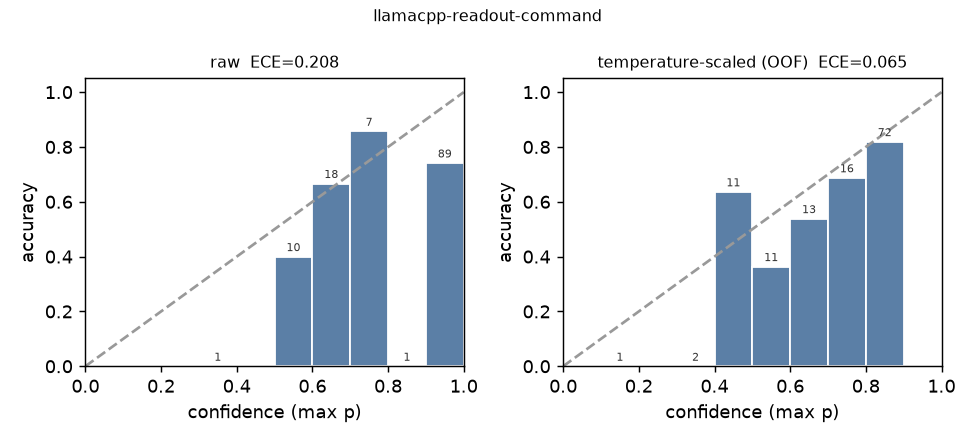
\includegraphics[width=.95\linewidth]{figures/reliability-readout-command.png}
\caption{Reliability diagrams of the readout's 24-way command answers on the held-out rows (bin counts above the bars). Left: raw next-token confidence sits at 0.9--1.0 with 74\% accuracy (ECE 0.208). Right: one temperature per fold, fitted on other seed requests (T$\approx$4.3), puts the bars on the diagonal (ECE 0.065); no answer clears 0.9 any more.}
\label{fig:reliability}
\end{figure}
\paragraph{The gate.} On the 939 pairs the readout reaches AUROC 0.952 (ECE 0.108$\to$0.030,
$T\approx6.4$). Synthetic negatives are nearly airtight: swapped operations are accepted 7.3\%
of the time, wrong ports never, and 1 of 156 dangerous swaps is accepted at $p>0.5$. On the
generative model's real calls (Table~\ref{tab:gate}) it flags 15 of the 20 command confusions
and 7 of the 13 diagnose-instead calls at $p<0.5$, false-flags 2 of the 10 format slips, and
false-flags 30 of the 151 correct calls (76 at $p<0.9$); AUROC on the real pairs alone is 0.714.
Prompt wording moves the raw operating point more than calibration does: an earlier phrasing of
the same question put mean $p(\text{yes})$ on correct proposals at 0.21 (AUROC 0.91) against
0.82 for the final phrasing (AUROC 0.95).

\begin{table}[t]\centering\footnotesize\setlength{\tabcolsep}{4pt}
\resizebox{\linewidth}{!}{%
\begin{tabular}{lrrrrr}
\toprule
backend & AUROC & ECE raw$\to$T & confusions flagged & correct false-flagged & dang.\ swaps accepted \\
\midrule
readout Qwen3-4B & 0.952 & 0.108$\to$0.030 & 15 / 20 & 30 / 151 & 1 / 156 \\
readout Qwen3.5-0.8B (no thinking) & 0.879 & 0.119$\to$0.047 & 13 / 20 & 36 / 151 & 25 / 156 \\
Laya 421M (0-shot) & 0.757 & 0.178$\to$0.022 & 1 / 20 & 1 / 151 & 101 / 156 \\
ft.\ ModernBERT-base, round 1 (held-out) & 0.647 & 0.107$\to$0.062 & 2 / 2 & 37 / 40 & 0 / 38 \\
ft.\ ModernBERT-base, gate-only (held-out) & 0.556 & 0.050$\to$0.087 & 1 / 2 & 14 / 40 & 8 / 38 \\
open-jev-deberta-v3-large (0-shot) & 0.668 & 0.403$\to$0.059 & 0 / 20 & 0 / 151 & 155 / 156 \\
openJev-verdict-2.0 (0-shot) & 0.566 & 0.284$\to$0.057 & 0 / 20 & 0 / 151 & 156 / 156 \\
NLI cross-encoder (0-shot) & 0.560 & 0.390$\to$0.058 & 0 / 20 & 10 / 151 & 144 / 156 \\
\bottomrule
\end{tabular}}
\caption{The gate question, ``does the proposed action do what the operator asked?'', at the
0.5 threshold after out-of-fold temperature scaling. Real pairs are the generative model's own
calls on the 195 paraphrases.}
\label{tab:gate}
\end{table}

\subsection{E2 --- open encoder decision models, zero-shot}

None transfers to the 23-command catalog. openJev-verdict-2.0 answers the 8-way tool question at
72.7\% (58.5\% with shortened descriptions) but returns the same label for every request on the
24-way command question; probing with 6, 12, 16, 20 and 24 options shows the collapse begins at
about six, consistent with its 5-candidate evaluation and with Laya's reported Banking77
weakness. open-jev-deberta-v3-large answers the command question at 70.8\% (bare option names,
one question per pass because of its 512-token context) and \texttt{is\_write} at 88.8\%, but
the tool question at 23.8\%. The NLI cross-encoder reaches 53.1\% / 86.5\%. All three are at
chance on the gate (Table~\ref{tab:gate}) and, being honest about it, abstain or spread their
mass: after scaling none accepts a dangerous swap above 0.9. Laya's typed-decisions checkpoint
is the strongest zero-shot encoder on all 519 rows (tool 61.7\%, command 51.4\%, \texttt{is\_write}
81.1\%, \texttt{touches\_poe\_power} 86.3\%) and its English checkpoint the strongest zero-shot
gate (AUROC 0.757, real pairs 0.710), yet it flags 1 of the 20 real confusions at $p<0.5$ and
accepts 101 of 156 dangerous swaps. On all 519 rows open-jev-deberta scores 31.6 / 45.1 / 75.3 /
39.7 and the NLI baseline 20.6 / 40.8 / 81.9 / 68.2.

\paragraph{A sub-1B decoder.} Qwen3.5-0.8B reads out nothing in its default template (the first
generated token opens a thinking block: label mass 0); with thinking disabled it reaches tool
74.6\%, command 35.0\%, \texttt{is\_write} 81.9\%, \texttt{touches\_poe\_power} 80.8\% on the 260
base rows with 71--84\% of the mass on the labels for the choice questions and a 95\% order-flip
rate on the tool question (rotation averaging: 68.8$\to$74.6\%). As a gate: AUROC 0.879, 13 of
20 real confusions flagged, 36 of 151 correct calls false-flagged, 25 of 156 dangerous swaps
accepted.

\subsection{E3 --- a fine-tuned 150M encoder}

ModernBERT-base trained for 4 epochs on 2,605 examples (the training groups' rows and paraphrases;
CE + Brier, augmentation 0.5) and evaluated packed on the 126 held-out rows: tool 70.6\%, command
65.1\% (65.9\% with alternatives), \texttt{is\_write} 81.7\%, \texttt{touches\_poe\_power}
82.5\%; 6 dangerous confusions, none above 0.9 confidence; \texttt{touches\_poe\_power} ECE
0.129$\to$0.015. The readout on the same 126 rows: 84.9 / 69.8 (73.0) / 90.5 / 96.0. Two
recipe findings: the span head is position-aware --- asked alone, a question trained in the
second slot drops from 55\% to 7\% --- so batteries must be evaluated as packed, or trained with
question-order shuffling; and the gate head, trained with a 1:2 positive:negative mix, learned
the prior (it accepts 6.7\% of gold proposals). A DeBERTa-v3-base run under the same recipe
diverged to NaN confidences under bf16 autocast (a known DeBERTa-v3 failure mode) and is not
reported.

\paragraph{Round 2.} Shuffling the question order in training (each training example emitted
once more with its four questions permuted) and training for 8 epochs changes the picture: on
the same 126 held-out rows the encoder reaches tool 88.1\%, command 77.8\% (79.4\% with
alternatives), \texttt{is\_write} 95.2\%, \texttt{touches\_poe\_power} 96.8\%, with ECE
0.047$\to$0.021 (tool) and 0.069$\to$0.058 (command); it is now the better router than the 4B
readout on every question, with 3 dangerous confusions (1 above 0.9 after scaling), at 126\,ms
per NOUL on the board's CPU (Table~\ref{tab:latency}). The gate does not follow: a dedicated model
trained on 2,080 class-balanced pairs for 6 epochs reaches AUROC 0.556 on held-out pairs (0.68 on
the real ones) and accepts 79\% of wrong-port proposals, which locates the failure --- the gate
requires matching the proposed port and value against the request, and this encoder does not
learn exact matching from two thousand synthetic pairs. The decoder readouts do.

\subsection{E4 --- latency}

Table~\ref{tab:latency}. The board runs the Snapdragon \texttt{llama-server} build CPU-only
beside the production NPU tenant (the binary links the Hexagon backend and aborts on the busy DSP
unless \texttt{GGML\_HEXAGON\_NDEV=0}); the encoders run under CPU torch in an isolated
environment. With the question legend prefix-cached, a readout router question costs
1.23--1.32\,s wall on six Kryo threads for 20 evaluated tokens ($\approx$16 tok/s incremental
prefill) and the gate question 3.1\,s for 52; a four-question battery is therefore $\sim$5\,s,
sequential, while one gate check per write is $\sim$3\,s. The fine-tuned 150M encoder answers one
NOUL in 126\,ms at four threads and the gate question in 183\,ms; its packed four-question battery
is a $\sim$1,100-token sequence and costs 2.5\,s. Co-tenancy costs nothing measurable: a
generative turn through the NPU runtime (96-token answer) took 4.43--4.52\,s idle and
4.32--4.33\,s while the CPU readout answered a continuous stream of questions.

\begin{table}[t]\centering\footnotesize\setlength{\tabcolsep}{4pt}
\begin{tabular}{llrrr}
\toprule
backend & host & 4-question battery & one NOUL & gate NOUL \\
\midrule
readout Qwen3-4B, prefix cached & QCS9075 CPU, 6 thr. & $\approx$5.1\,s & 1.24\,s & 3.1\,s \\
readout Qwen3-4B, prefix cached & Grace CPU, 12 thr. & $\approx$2.4\,s & 0.56\,s & 1.32\,s \\
fine-tuned ModernBERT-base & QCS9075 CPU, 4 thr. (1 thr.) & 2.51\,s (6.47) & 126\,ms (195) & 183\,ms (332) \\
fine-tuned ModernBERT-base & GB10 GPU & 12\,ms & 9\,ms & --- \\
Laya 421M & QCS9075 CPU, 4 thr. (1 thr.) & 3.37\,s (5.47) & 352\,ms (720) & 527\,ms (1199) \\
openJev-verdict 151M, torch (ONNX) & QCS9075 CPU, 4 thr. & 3.35\,s (4.75) & 295\,ms (361) & 337\,ms (429) \\
NLI DeBERTa-v3-base & QCS9075 CPU, 4 thr. & 5.15\,s & 274\,ms & 330\,ms \\
open-jev-deberta-v3-large & QCS9075 CPU, 4 thr. & 5.79\,s & 799\,ms & 982\,ms \\
\bottomrule
\end{tabular}
\caption{Median wall time per call. Encoder batteries answer all four questions in one packed
pass; the 24-option question dominates their length.}
\label{tab:latency}
\end{table}

\section{Serving-path reality}
\label{sec:serving}

The production runtime on the board (GenieX v0.4.0, compiled W4A16 bundle) answered a request
with \texttt{logprobs:true, max\_tokens:1} by returning \texttt{"logprobs": null}, three
generated tokens, and \texttt{cached\_tokens: 0}; the binaries of every GenieX version on hand
contain no \texttt{n\_probs} plumbing. On that path a typed decision collapses to a text label:
measured live on the 195 paraphrases, a 4-way text-label tool choice from the same 4B scored
88.7\% (75.4\% on indirect phrasing) against 93.3\% for its own tool call after format
normalization, and a 24-way command label 70.8\% against 83.1\%; 7\% of its answers changed
when the option order was reversed. Probabilities are available only through upstream
llama.cpp on the Hexagon backend --- built, not yet deployed, and unable to share the NPU with
the production tenant --- or on the CPU, where the readout and every encoder above run beside
the NPU agent. The CPU latency numbers in \S\ref{sec:experiments} are the operative ones.

\section{Discussion}

\paragraph{What the gate buys.} A generated tool call gives the human a command and a reason.
The gate question gives them a number whose meaning has been measured: at the 0.5 operating
point, three of four dangerous misreads carry a warning and one in five correct proposals does.
Whether that is the right point is a product decision --- the risk--coverage curve is in the
repository --- and the substantive change is that it \emph{is} a decision. Nothing here loosens
the gate; the design rule that no device write executes on a probability is kept.

\paragraph{Readout vs encoder.} On the router the fine-tuned encoder wins once its training
shuffles the question order: better on every question than the 4B readout on identical held-out
rows, calibrated as shipped, and forty times cheaper per question on the board's CPU. On the
gate only the decoder readouts work; every encoder variant, including one trained on balanced
gate pairs, stays near chance, and the wrong-port acceptance rate says why (exact port and value
matching is not learned from two thousand synthetic pairs). The division of labour on this class
of hardware is therefore concrete: an encoder for the per-turn router and pre-check
(milliseconds), a decoder readout for the per-write gate (seconds, once per confirmation), and
a llama.cpp server on the CPU beside the production runtime to serve the latter.

\paragraph{Calibration is measured, not assumed.} Every backend here was over-confident before
scaling, the readout's operating point moved by 0.6 between two phrasings of one question, and
the encoder's answers depended on where the question sat in the pack. The transferable rule is
procedural: label a few hundred of your own rows, group them by seed, fit the temperature
out-of-fold, and publish the reliability diagram beside the accuracy.

\paragraph{Limitations.} The authored rows and training paraphrases were LLM-generated and
LLM-verified; human review is pending and could move the adversarial numbers. There is one
domain and $N$ is in the hundreds, so per-style differences of a few points are within noise.
We could not run cloud Jev (no key); its published calibration is a vendor claim we neither
confirm nor dispute. The fine-tuning recipe is one configuration of one library; round 2 fixes
two identified defects rather than searching the space.

\section{Related work}

Jev and its documentation~\cite{jevblog,jevdocs,jevjagged}; open reproductions
\cite{openjevverdict,laya,openjevdeberta,openjev9b,openjevreadout} and the typed-decisions
benchmark~\cite{typeddecisions}; calibration of neural networks~\cite{guo2017} and of
instruction-tuned LMs; multiple-choice order sensitivity~\cite{zheng2023mcq,pezeshkpour2023};
zero-shot classification with NLI cross-encoders~\cite{yin2019}; selective
prediction~\cite{geifman2017}; tool-calling evaluation~\cite{bfcl}; the edge deployment this
work extends~\cite{lancefindings}.

\section{Conclusion}

The interface Jev popularised --- typed questions, a distribution per question, a confidence
axis --- can be served on an air-gapped board today, from the very model whose calls it checks,
and it gives a human confirm gate something it did not have: a calibrated, measured probability
that the proposed command is what the operator asked for. It does not make the small model a
better router, it is not calibrated until it is calibrated on the deployment's own rows, and it
costs seconds on a CPU. A 150M encoder fine-tuned on two thousand rows, with the question order
shuffled, out-routes it at a fortieth of the cost but cannot learn the gate. The dataset, code
and receipts are released so the next deployment can measure instead of assume.

\bibliographystyle{plain}
\bibliography{refs}

\end{document}
